\documentclass[12pt]{article}

\usepackage{multirow}
\usepackage{amsmath}
\usepackage{amsfonts}
\usepackage{float}
\usepackage{fancyhdr}
\usepackage{graphicx}
\usepackage{setspace}
\usepackage{subcaption}
\usepackage{booktabs}
\usepackage{bm}
\usepackage[colorlinks=true,linkcolor=blue, citecolor=red]{hyperref}
\usepackage{url}
\usepackage[top=.75in, left=.75in, right=.75in, bottom=1in]{geometry}
\usepackage[utf8]{vietnam}

% For algorithm
\usepackage{mathtools}
\usepackage{algorithm}
 \usepackage[noend]{algpseudocode}
 \usepackage{setspace, etoolbox, caption}

\usepackage{algpseudocode}


% ============ CODE ============
\usepackage{listingsutf8}%\usepackage{listings}
\usepackage{xcolor}
\definecolor{codegreen}{rgb}{0,0.6,0}
\definecolor{codegray}{rgb}{0.5,0.5,0.5}
\definecolor{codepurple}{rgb}{0.58,0,0.82}
\definecolor{backcolour}{rgb}{0.95,0.95,0.92}

% Styling for the code.
\lstdefinestyle{mystyle}{
    backgroundcolor=\color{backcolour},   
    commentstyle=\color{codegreen},
    keywordstyle=\color{magenta},
    numberstyle=\tiny\color{codegray},
    stringstyle=\color{codepurple},
    basicstyle=\ttfamily\footnotesize,
    breakatwhitespace=false,         
    breaklines=true,                 
    captionpos=b,                    
    keepspaces=true,                 
    numbers=left,                    
    numbersep=5pt,                  
    showspaces=false,                
    showstringspaces=false,
    showtabs=false,                  
    tabsize=2
}
\lstset{style=mystyle}

% Disable indentation on new paragraphs
%\setlength{\parindent}{0pt}

% Line spacing 1.5
\renewcommand{\baselinestretch}{1}

% Optional: graphic path
% \graphicspath{PATH_TO_GRAPHIC_FOLDER}

% To use Times font family, uncomment this row
% \usepackage{mathptmx}

% To use roman section / subsection, uncomment these rows
% \renewcommand{\thesection}{\Roman{section}}
% \renewcommand{\thesubsection}{\thesection.\Roman{subsection}}

% Define course name, report name and report title.
\newcommand{\coursename}{Phương pháp Toán cho Trí tuệ nhân tạo}
\newcommand{\reportname}{CLIP (Contrastive Language-Image Pretraining)}
\newcommand{\reporttitle}{Tóm tắt Final Project}
\newcommand{\studentname}{Nguyễn Đình Hà Dương (23122002)\\Nguyễn Lê Hoàng Trung (23122004)\\Đinh Đức Tài (23122013)\\Hoàng Minh Trung (23122014)}
\newcommand{\teachername}{TS. Cấn Trần Thành Trung\\ThS. Nguyễn Ngọc Toàn}

\newcommand{\leftfooter}{\LaTeX\ by \href{https://github.com/ductai05}{Duc Tai Dinh}}

% ============ HEADER AND FOOTER ============
% Header length
\setlength{\headheight}{29.43912pt}

% Footer page number would be on the lower-right corner
\pagestyle{fancy}
\fancyfoot{}
\fancyfoot[R]{Trang \thepage}

\lhead{CLIP: Connecting text and images}
\rhead{
Trường Đại học Khoa học Tự nhiên - ĐHQG HCM\\
\coursename
}
\lfoot{\leftfooter}

% ============ DOCUMENT ============
\begin{document}
\begin{titlepage}
\newcommand{\HRule}{\rule{\linewidth}{0.5mm}}
\centering

\textsc{\LARGE đại học quốc gia tphcm}\\[1.5cm]
\textsc{\Large trường đại học khoa học tự nhiên}\\[0.5cm]
\textsc{\large khoa công nghệ thông tin}\\[0.5cm]
\textsc{AI23 (23TNT1), FIT@HCMUS-VNUHCM}\\[0.5cm]

\HRule \\[0.4cm]
{ 
\huge{\bfseries{\reporttitle}}\\[0.5cm]
\large{\bfseries{Đề tài: \reportname}}
}\\[0.4cm]
\HRule \\[0.5cm]

\textbf{\large Môn học: \coursename}\\[0.5cm]

\begin{minipage}[t]{0.5\textwidth}
\begin{flushleft} \large
\emph{Sinh viên thực hiện:}\\
\studentname
\end{flushleft}
\end{minipage}
~
\begin{minipage}[t]{0.4\textwidth}
\begin{flushright} \large
\emph{Giáo viên hướng dẫn:} \\
\teachername
\end{flushright}
\end{minipage}\\[1.5cm]

{\large \today}\\[0.5cm]


\includegraphics[scale=.3]{img/hcmus-logo.png}\\[1cm] 

\vfill
\end{titlepage}
	
	
% \tableofcontents
\pagebreak

\section{Tóm tắt}

\paragraph{}{Chúng tôi lựa chọn \textbf{Hướng 2: Nghiên cứu một bài báo khoa học} với lý do sau:}

\begin{itemize}
    \item Nâng cao hiểu biết về các mô hình cơ bản, quan trọng trong lĩnh vực Machine learning / Deep learning / AI. 
    \item Hiểu cách ứng dụng của toán học và kĩ thuật lập trình trong nghiên cứu và thực tế.
    \item Tăng khả năng tự nghiên cứu và áp dụng tri thức mới vào thực tiễn.
    \item Nâng cao tư duy phản biện, phân tích, tổng hợp.
\end{itemize}

\paragraph{}{\textbf{CLIP} \cite{radford2021learning} (Contrastive Language-Image Pre-Training) là một mạng nơ-ron được huấn luyện trên nhiều cặp dữ liệu (ảnh, văn bản). Mô hình này có thể được hướng dẫn bằng ngôn ngữ tự nhiên để dự đoán đoạn văn bản phù hợp nhất với một hình ảnh, mà không cần được tối ưu hóa trực tiếp cho nhiệm vụ đó — tương tự như khả năng “zero-shot” (không cần huấn luyện lại) của GPT-2 và GPT-3.

CLIP đạt hiệu suất tương đương với ResNet-50 gốc trên bộ dữ liệu ImageNet theo cách “zero-shot”, mà không cần sử dụng bất kỳ ví dụ có gán nhãn nào trong 1,28 triệu ảnh ban đầu, từ đó vượt qua một số thách thức lớn trong lĩnh vực thị giác máy tính.

CLIP \cite{radford2021learning}, Code \cite{code_clip}, Blog \cite{blog_clip}.
}

\paragraph{}{\textbf{Lý do lựa chọn bài báo:}}

\begin{itemize}
    \item CLIP là một mô hình cơ sở (foundation model) quan trọng trong lĩnh vực học đa phương thức, kết nối giữa thị giác máy tính và xử lý ngôn ngữ tự nhiên.
    \item CLIP có ứng dụng đa dạng: truy vấn hình ảnh bằng văn bản; phân loại hình ảnh zero-shot và fewshot; phân tích nội dung video.
    \item CLIP được xây dựng dựa trên các kiến thức nền tảng toán học như đại số tuyến tính, xác suất thống kê. Hiểu rõ CLIP sẽ nâng cao kiến thức về toán học.
\end{itemize}

\paragraph{}{\textbf{Kế hoạch thực hiện:}}

\begin{enumerate}
    \item Phân tích các nền tảng của CLIP: Contrastive learning, Vision Transformer/Transformer, Embedding Vector Space,...
    \item Phân tích dữ liệu, cách huấn luyện CLIP, so sánh các mô hình.
    \item Các mô hình SOTA được phát triển thêm dựa trên CLIP: BLIP-2, BLIP3-o,... 
    \item Ứng dụng của CLIP vào cuộc thi truy vấn AI Challenge HCMC 2025.
\end{enumerate}
% \input{content/02-cpu}
% \input{content/08-ketluan} % 0

\newpage
\bibliographystyle{unsrt}
\bibliography{ref/ref}

% \appendix
% \section{Phụ lục}

\begin{figure}[H]
    \centering
    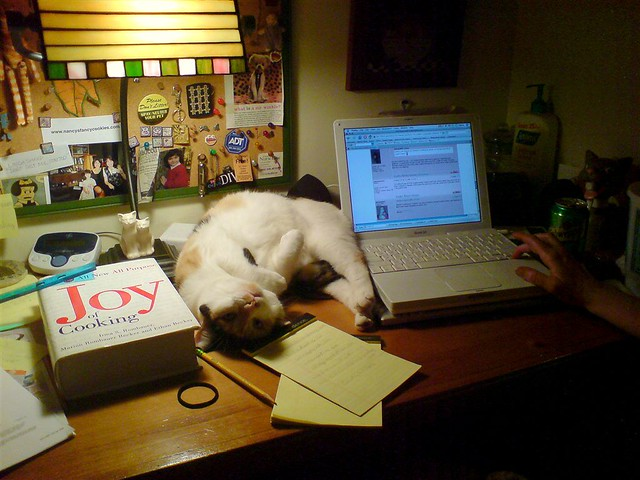
\includegraphics[width=0.75\linewidth]{appendix/cat-image.png}
    \caption{Hình ảnh một con mèo nằm giữa một cuốn sách và một cái laptop, trên một cái bàn nhỏ.}
\end{figure}


\begin{table}[H]
\centering
\begin{tabular}{|l|l|l|}
\hline
Văn bản cho trước           & \textbf{CLIP} & \textbf{ALIGN} \\ \hline
'a photo of a cat' & 0.0228        & 0.0018         \\ \hline
'a photo of a dog'          & 0.0020        & 0.0000         \\ \hline
\begin{tabular}[c]{@{}l@{}}'cat lying between \\ laptop computer and \\ book on small desk'\end{tabular} & 0.9752 & 0.9982 \\ \hline
\end{tabular}
\caption{Kết quả so sánh độ tương đồng ảnh-văn bản bởi CLIP và ALIGN}
\label{tab:CLIP-ALIGN}
\end{table}

\begin{table}[H]
\centering
\begin{tabular}{|l|l|}
\hline
Tác vụ                                                                    & \textbf{BLIP} \\ \hline
\begin{tabular}[c]{@{}l@{}}Tạo chú thích ảnh \\ (Image Captioning)\end{tabular} & \begin{tabular}[c]{@{}l@{}}a cat is sleeping on a \\ desk with a laptop\end{tabular} \\ \hline
\begin{tabular}[c]{@{}l@{}}How many cats are there? \\ (VQA)\end{tabular} & 1             \\ \hline
\begin{tabular}[c]{@{}l@{}}What is the cat's color?\\ (VQA)\end{tabular}  & white         \\ \hline
\end{tabular}
\caption{Kết quả của BLIP cho 2 tác vụ: VQA và Image Captioning}
\label{tab:BLIP}
\end{table}


\end{document}